% !TEX encoding = UTF-8 Unicode
\documentclass[../天体物理基础.tex]{subfiles}
\begin{document}
\section{宇宙学}
\subsection{基本认知}
奥伯斯佯谬:宇宙无限,恒星分布均匀,那么夜晚天空应该像白天一样明亮。考虑球壳中恒星发光
\begin{equation}
E=\int_{0}^{\infty}\frac{L}{4\pi r^{2}}\times n\times4\pi r^{2}\symup{d}r\to\infty.
\end{equation}
其中$n$是恒星数密度,有几种解释:恒星寿命有限;宇宙不是无限的;宇宙小尺度不是均匀的;宇宙年龄有限,遥远的星光还未到达我们;有星际消光存在;宇宙在膨胀光子发生红移;宇宙膨胀过快,光子无法到达。

宇宙充满物质,减速膨胀;没有物质,匀速膨胀。早期宇宙由辐射主导,后期物质主导,现在暗能量主导。

$\Omega_{0}>1$,束缚(封闭)宇宙,先膨胀后收缩

$\Omega_{0}<1$,开放宇宙,无限膨胀

$\Omega=1$,临界束缚,无限膨胀

\subsection{观测宇宙学}
观测宇宙时要假定一个相对 comoving 坐标系没有速度的 fundamental observer。它们的时间是 cosmic epoch, 也就是第一章提到的形如$\dfrac{2}{3H_{0}}$的时间。

我们可以根据球状星团年龄和放射性半衰期来确定宇宙年龄下限。

对高红移\uppercase\expandafter{\romannumeral 1}a 观测表明,它们的距离比预期的更高,因此宇宙正在加速膨胀,存在暗能量。

微波背景辐射 CMB 观测结果给出宇宙年龄$13.7\pm\qty{0.2}{Gyr}$。

物质含量可通过旋转曲线、星系团内部热气体辐射功率、引力透镜、近期轻元素丰度对原初核合成限制等确定。此外,物质、辐射、曲率、暗能量不同占比会影响 CMB 功率谱,也可作为限制。

由于太阳的运动,CMB 相对我们有一多普勒偶极不对称性,相对背景量级在$10^{-3}$.扣除此效应和星系前景辐射,CMB 各向异性$\dfrac{\Delta{}T}{T}$仅有$10^{-5}$量级的变化。

这个各向异性来自声波振荡:引力和光压的相互作用导致等离子体在引力势中振荡。只要物质和辐射之间有耦合,物质分布中的微小扰动都会被光子的扩散所牵制,发生粘滞性衰减。物质和辐射解耦,物质变为独立后,质量稍有超出的区域,其范围就会由于对周围的引力作用而增长。因此 CMB 功率谱携带了早期宇宙结构的信息。CMB 中热点和冷点在天空中角距离尺度为$\ang{1;;}$左右。

\subsection{暴胀 Inflation}
主要有两个问题。第一,我们认为波动的波长大于视界时就没有物理机制能破坏波动中蕴藏的信息。大一统时代的视界约$\qty{3e-26}{cm}$,宇宙尺度$\qty{3}{cm}$,按理说宇宙这头和那头应该完全没关系了,CMB 却高度各向同性,粒子如何达成信息交换?第二点,宇宙过于平直了。

宇宙起源于一个极小的区域,在暴胀前宇宙的大小远小于视界大小,物质耦合在一起,足以达到玻尔兹曼统计平衡,因而具有相同的温度。很快宇宙指数级膨胀,再高的山脉和地球比起来都微不足道,因此宇宙被拉平了。同时原先平衡的信息被拉到了视界尺度之外,一直留存了下来,保存到今天。

$\qty{e-36}{s}$宇宙高度对称。
$\qty{e-35}{s},T<\qty{e28}{K}$,强互作用分离,对称性破缺,宇宙真空有很高的能量。
$10^{-35}\text{\textendash}\qty{e-32}{s}$,宇宙指数膨胀,尺度增大$10^{50}$倍。

\subsection{热历史}
pass 这部分时标可能有点问题。

我们假设$T>\dfrac{m\symup{c}^{2}}{k}$时质量为$m$的$A$粒子就变成相对论性。这个温度之上正反$A$粒子就能湮灭产生光子,反之光子也能生成$A$粒子。随着宇宙不断膨胀,温度不断降低,正反物质不断湮灭成光子。不过由于正物质比反物质多十亿分之一,所以没有完全湮灭。

我们用一个指标$T_{10}$来描述某一温度$T_{10}\times\qty{e10}{K}$对应的宇宙年龄$\tau$和反应时标。由于
\begin{equation}
\frac{a}{a_{0}}=\left(\frac{32\pi\symup{G}}{3\symup{c}^{2}}U_{0}\right)^{\frac{1}{4}}\tau^{\frac{1}{2}},
\end{equation}
因此
\begin{equation}
\tau=\left(\frac{32\pi\symup{G}}{3\symup{c}^{2}}U\right)^{-\frac12}\sim T_{10}^{-2}\,\unit{s}.
\end{equation}

如同化学反应一样,物质湮灭和转化的速率依赖于温度和数密度,但宇宙在不断膨胀,如果膨胀速率超过了反应速率,物质间将不再能相互作用,便会维持最后的相对占比,我们称其为 freeze out.

电子扮演光子和中微子间的中介。中微子反应时标为$\tau=160T_{10}^{-5}\,\unit{s}$,因此温度下降到一定程度时反应就会中止,此时$T_{10}^{2}\,\unit{s}=160T_{10}^{-5}\,\unit{s}$,中微子 freeze out,散射出去,成为中微子背景。不过电子还会和光子相互作用,因此 CMB 的温度比中微子背景温度更高一点,前者$\qty{2.7}{K}$,后者$\qty{1.9}{K}$.

质子会转化成中子,时标$\tau\sim T_{10}^{-5}\,\unit{s}$,因此$T=\qty{e10}{K},\tau=\qty{1}{s}$时冻结。中子和质子的比大概 0.22.不过实际冻结时间会晚一点,因为电子湮灭反应在$T_{10}=0.5$的时候才停止,期间提供了一些能量。

孤立中子会衰变成质子,但此时有大量的中子和质子,理论上可以进行核合成。此时的问题是高能光子会打碎氘,而$T<\qty{e9}{K},\tau>\qty{100}{s}$时光子能量才降低到足够的地步,因此主要是氦残留下来
\begin{equation}
Y=2\frac{\ce{n}/\ce{p}}{1+\ce{n}/\ce{p}}\sim0.36.
\end{equation}
考虑到冻结修正和$\beta$衰变,实际 0.24.

\subsection{微波背景辐射}
早期炽热宇宙冷却,残留热辐射红移至微波波段,高度各向同性的$\qty{2.73}{K}$黑体辐射。

偶极不对称性:太阳相对哈勃流运动引起的涨落,太阳朝向和背向温度变化约$10^{-3}$,$\Delta T=\qty{3.353}{mK}$

扣除银河系尘埃辐射和偶极不对称性有十几万分之几$\unit{K}$变化,表明宇宙演化早期有微小的不均匀性,导致星系形成。

Sunyaev-Zel'dovich 效应:CMB 光子被星系团热气体中高能电子散射到高频波段,导致 CMB 能谱改变。如果星系团相对于 CMB 静止参考系存在一个本动速度,也会导致 CMB 辐射强度的变化。运动学 S-Z 效应比热 S-Z 效应弱。

结合 X 射线观测确定 Hubble 常数和利用星系团的 S-Z 效应计数可以确定角直径距离、限制宇宙学基本参量、研究星系团的演化。从而最终限制宇宙学模型。

宇宙线是十分高能的。高速粒子 ($\qty{e20}{eV}$) 与 CMB 光子反应,因此能量高于一定程度的宇宙线并不存在,观测中会发现 Greisen-Zatsepin-Kuzmin cutoff.

早期宇宙引力倾向于使重子成团,光子则倾向于消除各向异性。二者的相互作用导致等离子体在引力势中振荡。这种振荡产生的温度和密度变化被记录下来。宇宙膨胀,光子平均自由程增大,微波背景辐射小范围衰减,因此振动频谱记录了温度涨落和宇宙结构。

光子持续和电子发生康普顿散射,使$T_{\text{matter}}\sim T_{\text{radiation}}$,直到$z\sim1500$温度小于$\qty{13.6}{eV}$.引入电离度
\begin{equation}
\chi\left(z\right)=\qty{3.4e-3}{}\frac{\left(\Omega_{\text{m}}h_{70}^{2}\right)^{\frac{1}{2}}}{\Omega_{\text{b}}h_{70}^{2}}\left(\frac{z}{1000}\right)^{12.75}=0.04\left(\frac{z}{1000}\right)^{12.75},
\end{equation}
计算光深
\begin{equation}
\tau\left(z\right)=\int_{0}^{z}n_{{\color{blue}{\ce{e}}}}\left(z\right)\chi\left(z\right)\sigma_{\text{T}}\frac{\symup{d}l}{\symup{d}z}\symup{d}z.
\end{equation}
$n_{{\color{blue}{\ce{e}}}}$和$\dfrac{\symup{d}l}{\symup{d}z}$依赖于$\Omega_{\text{b}},\Omega_{\text{m}}$和$h_{70}^{2}$,因此积分结果最后只和$z$有关
\begin{equation}
\tau\left(z\right)=0.37\left(\frac{z}{1000}\right)^{14.25}.
\end{equation}
散射概率为$P=\symup{e}^{-\tau}$,最终散射概率密度分布为
\begin{equation}
P'\left(z\right)\symup{d}z=-\frac{\symup{d}P}{\symup{d}z}\symup{d}z=\symup{e}^{-\tau}\frac{\symup{d}\tau}{\symup{d}z}\symup{d}z.
\end{equation}
这近似高斯分布,峰值$z=1065,\sigma_{z}\sim80$,大部分 CMB 光子来自$950<z<1100$,大约大爆炸后 37 万年。值得注意的是此时电离度只有 0.09. 其功率峰值粗略对应于光子{}-{}重子流体脱耦时的振荡特征。峰值位置反映了宇宙曲率,重子密度,暗物质密度。再电离时期对 CMB 光深的贡献只有 0.06. CMB $10^{-5}$级别的波动告诉我们绝热扰动、多普勒运动和引力红移的影响,角度$\ang{1;;}$时候扰动最大,因此现在观察 CMB 背景可以看到角距离 $\ang{1;;}$的峰值和峰谷。

\begin{figure}[!htp]
\centering
\tikzset{every picture/.style={line width=0.75pt}}
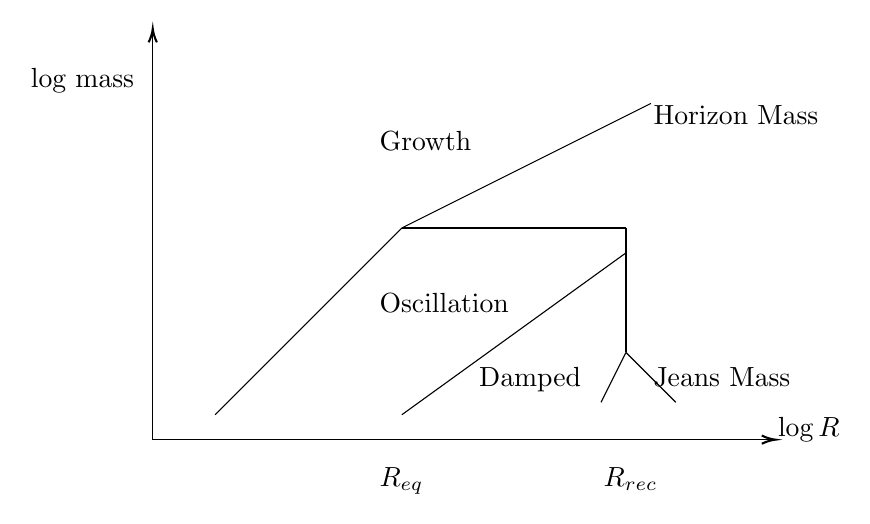
\begin{tikzpicture}[x=0.5pt,y=0.5pt,yscale=0.9,xscale=0.9]
\draw (0,30) -- (0,360) ;
\draw [shift={(0,360)},rotate=270][line width=0.75](10.93,-3.29) .. controls (6.95,-1.4) and (3.31,-0.3) .. (0,0) .. controls (3.31,0.3) and (6.95,1.4) .. (10.93,3.29); 
\draw (0,30) -- (500,30) ;
\draw [shift={(500,30)},rotate=180][line width=0.75](10.93,-3.29) .. controls (6.95,-1.4) and (3.31,-0.3) .. (0,0) .. controls (3.31,0.3) and (6.95,1.4) .. (10.93,3.29); 
\draw (50,50) -- (200,200) ;
\draw (200,200) -- (400,300) ;
\draw (200,200) -- (380,200) ;
\draw (200,200) -- (380,200) ;
\draw (380,200) -- (380,100) ;
\draw (200,50) -- (380,180) ;
\draw (380,100) -- (360,60) ;
\draw (380,100) -- (420,60) ;
%Text
\draw (-100,330) node [anchor=north west][inner sep=0.75pt]   [align=left] {log mass};
\draw (500,50) node [anchor=north west][inner sep=0.75pt]   [align=left] {$\log R$};
\draw (180,10) node [anchor=north west][inner sep=0.75pt]   [align=left] {$R_{\text{eq}}$};
\draw (360,10) node [anchor=north west][inner sep=0.75pt]   [align=left] {$R_{\text{rec}}$};
\draw (180,280) node [anchor=north west][inner sep=0.75pt]   [align=left] {Growth};
\draw (400,300) node [anchor=north west][inner sep=0.75pt]   [align=left] {Horizon Mass};
\draw (180,150) node [anchor=north west][inner sep=0.75pt]   [align=left] {Oscillation};
\draw (260,90) node [anchor=north west][inner sep=0.75pt]   [align=left] {Damped};
\draw (400,90) node [anchor=north west][inner sep=0.75pt]   [align=left] {Jeans Mass};
\end{tikzpicture}
\captionsetup{justification=raggedright, singlelinecheck=false}
\caption{金斯质量随时间的变化。}
\label{model}
\end{figure}

在大尺度结构的观测上,另一个重要的方向是重子声波振荡 (Baryon Acoustic Oscillations). 在宇宙的光子退耦前,物质在引力的作用下向内收缩,而又在物质压强下向外扩张,从而形成了声波振荡。辐射主导时期,声速可以达到$\dfrac{\symup{c}}{\sqrt{3}}$,直到物质主导 ($z\approx3300$),共动声学视界在$R_{\text{s}}\sim\qty{150}{Mpc}$冻结。我们称共动声学视界包裹的质量为 Horizon Mass. 再失去光子支撑后,如此巨大的质量应该会一定程度上坍缩,因此 Jeans 质量低于 Horizon Mass. Recombination 时 Jeans 长度比视界尺度大得多,因此我们预计在所有亚视界尺度上都会有流体振荡,包括 Recombination 时刚好进入视界的尺度。视界尺度上流体的动力学将转化为宇宙微波背景辐射功率谱中的第一个声学峰。它的位置反应了宇宙的曲率,高度反应了重子物质含量。第二个和第三个峰值分别详细说明了正常物质和暗物质的密度。一般物质越多,辐射{}-{}物质密度相等时刻越靠前,整体振荡就越弱。

除此之外,光子和电子的相互作用会把小尺度结构 smooth 掉,也就是 Silk damping 区域。

直到 Recombinaiton 后,光子电子彻底退耦,Jeans 质量才掉到$\qty{e6}{M_{\odot}}$.

张量扰动能影响 CMB 偏振全部分量,标量扰动只能影响部分。

我们可以想办法描述这种振荡的演化。定义扰动场$\delta{}\left(\vec{x}\right)$,进行 Fourier 变换
\begin{align}
\delta{}\left(\vec{x}\right)&=\frac{1}{\left(2\pi\right)^{\frac32}}\int\delta{}\left(\vec{k}\right)e^{-i\symbf{k}\cdot\symbf{x}}\symup{d}^{3}\vec{k}.\\
\delta{}\left(\vec{k}\right)&=\frac{1}{\left(2\pi\right)^{\frac32}}\int\delta{}\left(\vec{x}\right)e^{i\symbf{k}\cdot\symbf{x}}\symup{d}^{3}\vec{x}.
\end{align}
定义物质扰动满足
\begin{align}
&\frac{\delta{}\rho}{\rho_{0}}=\delta{}\left(t\right)e^{i\symbf{k}\cdot\symbf{r}}.\\
&\frac{\symup{d}^{2}\delta{}}{\symup{d}t^{2}}+2\left(\frac{\dot a}{a}\right)\frac{\symup{d}\delta{}}{\symup{d}t}-\delta{}\left(4\pi\symup{G}\rho_{0}-k^{2}c_{\text{s}}^{2}\right)=0.\label{6.5.4}
\end{align}

对于小扰动,忽略声波,考虑纯物质宇宙
\begin{equation}
4\pi\symup{G}\rho_{0}=\frac{2}{3t^{2}},\frac{\dot a}{a}=\frac{2}{3t},
\end{equation}
(\ref{6.5.4}) 式变为
\begin{equation}
\frac{\symup{d}^{2}\delta{}}{\symup{d}t^{2}}+\frac{4}{3t}\frac{\symup{d}\delta{}}{\symup{d}t}-\frac{2}{3t^{2}}\delta{}=0.
\end{equation}
取试探解$\delta{}=at^{n}$,代入得到
\begin{equation}
n_{1}=\frac{2}{3},n_{2}=-1.
\end{equation}
只有$\dfrac{2}{3}$符合物理。因此
\begin{equation}
\delta{}_{k}=\delta{}_{k,0}\left(\frac{t}{t_{0}}\right)^{\frac{2}{3}}=\delta{}_{k,0}\left(\frac{a}{a_{0}}\right).
\end{equation}

曲率为主的宇宙,
\begin{equation}
\frac{\symup{d}^{2}\delta{}}{\symup{d}t^{2}}+\frac{2}{t}\frac{\symup{d}\delta{}}{\symup{d}t}=0.
\end{equation}
解只有$n=0,-1$,即扰动不能增长。

辐射主导时,
\begin{equation}
\frac{\symup{d}^{2}\delta{}}{\symup{d}t^{2}}+2\left(\frac{\dot a}{a}\right)\frac{\symup{d}\delta{}}{\symup{d}t}-\delta{}\left(\frac{32}{3}\pi{}\symup{G}\rho-k^{2}c_{\text{s}}^{2}\right)=0.
\end{equation}
考虑到$a\propto{}\tau^{\frac{1}{2}}$,
\begin{equation}
\delta{}_{k}=\delta{}_{0}\left(\frac{a}{a_{0}}\right)^{2}.
\end{equation}
物质扰动不增长,因此不会坍缩,Jeans 质量会一直增长,符合之前的描述。

小尺度的扰动进入视界时间早,如果仍然为辐射为主,扰动基本不能增长。

大尺度的扰动在物质为主时进入视界,扰动随尺度因子线性增长。

\subsection{暗物质与大尺度结构的形成}
Recombination 前,辐射和正常(重子)物质是耦合在一起的。如果星系起源于宇宙早期正常物质的密度涨落,这种涨落也应该造成 CMB 的涨落。但我们知道 CMB 扰动仅有$10^{-5}$,如此密度不足以在已有的时间内形成星系和星系团。况且 silk damp 的存在,Jeans 质量高于星系质量,为什么现在有星系?

因此,我们相信,暗物质的密度涨落应该在宇宙大尺度结构的形成中起主要作用。暗物质不会相互反应,金斯质量为零,也没有声震荡。宇宙开始包含均匀分布的暗物质和正常物质。大爆炸后数千年暗物质开始成团。暗物质确定宇宙中物质的总体分布和大尺度结构。正常物质在引力作用下向高密度区域聚集,形成星系和星系团。

为什么不可能源于重子物质密度涨落?

1. 脱耦前光子阻碍物质收缩;

2. 涨落引起的变化在微波背景辐射仅表现为千分之一变化;

3. 微波背景辐射记录的物质密度不足以在$100$亿年内形成星系。

因此,暗物质起主要作用,它与辐射场不耦合,密度涨落也不会引起微波背景辐射变化

暗物质只参与弱作用和引力相互作用,与辐射场不耦合,因此暗物质的凝聚可以在辐射与正常物质脱耦前发生。(当然实际上有暗物质相互碰撞产生光子的模型,详情请见 Chapter 3.4 in \textit{Modern Cosmology} by Scott Dodelson)暗物质的不均匀分布产生的引力变化导致微波背景辐射微小起伏。

暗物质的成分(根据退耦时刻粒子的能量与其静止质量相比较来区分):

热暗物质 (HDM):粒子质量很小,速度接近光速(如中微子),影响大尺度结构。

冷暗物质 (CDM):粒子质量较大、速度较慢,影响小尺度结构。

暗物质很可能同时包括热暗物质和冷暗物质。

宇宙中 90\%以上的质量来自暗物质。

%\printbibliography

\end{document}